\chapter{Introduction}\label{C:intro}

\subsection{The reinforcement learning problem}

Reinforcement learning is a framework of learning that describes how an agent learns by interacting with the environment. The framework involves 2 entities the agent and environment. The agent is only entity that we as designers have direct control of. We decide how its learns and decides on its actions. The environment is the context and situation that the agent is in. There are three important flows of information;  the state of the environment to the agent, the action decision to the environment and lastly the reward to the agent. This can be best be understood in the figure below.

\begin{fig}
\begin{center}
    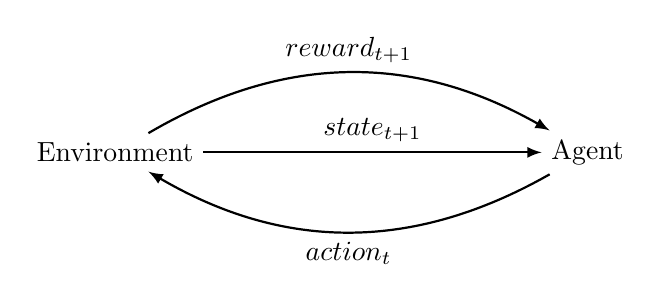
\begin{tikzpicture}[
        node distance=6cm, % Increased node distance for better spacing
    ]
        % Define nodes
        \node (env) {Environment};
        \node (agent) [right of=env] {Agent};

        % Define arrows and labels without boxes
        \draw [-latex,bend left, thick] (env) edge node[anchor=south] {$reward_{t+1}$} (agent);
        \draw [-latex, thick] (env) -- node[anchor=south] {$state_{t+1}$} (agent);
        \draw [-latex,bend left,thick] (agent) edge node[anchor=north] {$action_{t}$} (env);
    \end{tikzpicture}
    \caption{The flow of information between th environment and agent}
\end{center}
\end{fig}

The state is a representation of the information within the environment that the agent will use to make its decision on which action to take. The reward signal is treated as the final word on how good the situation is, the more reward the better, always. Lastly the action is sent to the environment and the environment will in turn return the next state that the action has taken the agent. This brings us to the reinforcement learning problem which can be framed as such "How does the agent decide which actions to take given the state such that it maximises the future cumulative reward". It is important that the agent maximises all *future cumulative* reward otherwise short term gains could be made to the sacrifice of larger long term gains. This idea has been formalised by Richard Sutton as the reward hypothesis

\begin{quote}
    "That all of what we mean by goals and purposes can be well thought of as maximization of the expected value of the cumulative sum of a received scalar signal (reward)." 
    \cite{suttonReinforcementLearningSecond2018}
\end{quote}

\subsection{Formalism}

The reinforcement problem can be formalised as a Markov Decision Process. The MDP is a collection of states, actions and rewards along with a transition function which states that probability of the next reward and state given a state and reward.
$$
Pr\left\{ S_{t}=s', R_{t}=r | S_{t-1}=s, A_{t-1}=a \right\} 
$$
This function completely characterises the dynamics of the environment. This abstraction of the environment to a MDP is widely applicable and serves as the basis for much of reinforcement learning.  We can see here that transition function only looks at the previous state. It can do this because we assume that the state representation has the *Markov property* [@suttonReinforcementLearningSecond2018], which states including previous states in the conditional wont change the probability as the current state will have already captured that information. In interaction with the agent the MDP will generate a sequence that looks like:
$$S_{1},A_{1},R_{2},\dots S_{n},A_{n}, R_{n+1},\dots$$
In the case above we have an infinite sequence and these are continuing tasks as they have no end. Alternatively you could have episodic tasks that have a start and ending with a terminal state.
"The cumulative sum of a received scalar signal" part of the reward hypothesis can be formalised to be the return $G$.
$$
G_{t}=R_{t+1}+\gamma R_{t+2}+\gamma^{2}R_{t+3}\dots=\sum_{k=t}^{\infty}\gamma^{t-1}R_{t+1}
$$

$\gamma$ is called the discounting factor. It is usually added for two reasons. Firstly because it means that the return won't be infinite which simplifies it mathematically. Secondly is due to the very natural intuition that the future is less predicable than the present, thus more distance rewards should have less weight as they are less certain. 


A decision agent will use policy $\pi$ which provides the probability of taking action $a$ given state $s$. This policy could be deterministic or stochastic.
To get the policy the agent needs an understanding of value of its current state. This is called the value function and it is a expectation of the future rewards.
$$
v_{\pi}(s)=\mathbb{E}\left[ G_{t}| S_{t}=s\right] 
$$
The value function depends on the state, policy and discounting factor $\gamma$. In a similar vain to value function we have the action-value function which is the expected future reward given a state and action taken.

$$
q_{\pi}(s,a) = \mathbb{E}\left[ G_{t} | S_{t}=s, A_{t}=a \right] 
$$

These functions are closely related and have a large amount of connected definitions this one:

$$
q_{\pi}(s,a)=\mathbb{E}\left[ R_{t+1}+\gamma v_{\pi}(S_{t+1})|S_{t}=s, A_{t}=a \right] 
$$

The maximising part of the reinforcement problem can be solved by the finding optimal actions. We can define both $v_{\star}=\underset{ \pi }{ \text{max} }\ v_{\pi}(s)$ and $q_{\star}=\underset{ \pi }{ \text{max} }\ q_{\pi}(s,a)$ as the optimal value given optimal actions afterwards.
If we can find $q_{\star}$ then the problem is solved as we could make a policy $\pi_{\star}$ that is greedy with respect to $q_{\star}$. 

This form explicitly learning a value function then implicitly getting a full policy or just needed actions from it is called value based methods. Alternatively you can learn the policy directly with policy based methods. The effectiveness of these methods depend heavily on how easy the value function or policy is to learn.